\begin{frame}[fragile]{The \texttt{map} problem: natural implementation}
\begin{adjustwidth}{-1.2em}{-1.2em}
\begin{lstlisting}
let rec %\textcolor{red}{map}% f xs =
  match xs with
  | [] ->
      []
  | x :: xs ->
      let y = f x in
      %\textcolor{cyan}{y ::}% %\textcolor{red}{map}% f xs
\end{lstlisting}
\vfill
\begin{lstlisting}
# List.init 250_000 (fun _ -> ())
  |> map Fun.id
  |> ignore
  ;;
Stack overflow during evaluation (looping recursion?).
\end{lstlisting}
\end{adjustwidth}
\end{frame}

\begin{frame}{The \texttt{map} problem: natural implementation}
\centering
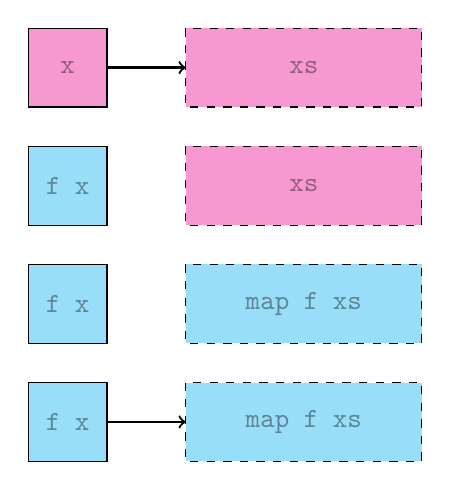
\begin{tikzpicture}[yscale=-1]
    \draw [fill=magenta, fill opacity=0.4] (0,0) rectangle (1,1) node [pos=.5] {\texttt{x}} ;
    \draw [fill=magenta, fill opacity=0.4, dashed] (2,0) rectangle (5,1) node [pos=.5] {\texttt{xs}} ;
    \draw [thick, ->] (1,0.5) -- (2,0.5) ;
    
    \draw [fill=cyan, fill opacity=0.4] (0,1.5) rectangle (1,2.5) node [pos=.5] {\texttt{f x}} ;
    \draw [fill=magenta, fill opacity=0.4, dashed] (2,1.5) rectangle (5,2.5) node [pos=.5] {\texttt{xs}} ;
    
    \draw [fill=cyan, fill opacity=0.4] (0,3) rectangle (1,4) node [pos=.5] {\texttt{f x}} ;
    \draw [fill=cyan, fill opacity=0.4, dashed] (2,3) rectangle (5,4) node [pos=.5] {\texttt{map f xs}} ;
    
    \draw [fill=cyan, fill opacity=0.4] (0,4.5) rectangle (1,5.5) node [pos=.5] {\texttt{f x}} ;
    \draw [fill=cyan, fill opacity=0.4, dashed] (2,4.5) rectangle (5,5.5) node [pos=.5] {\texttt{map f xs}} ;
    \draw [thick, ->] (1,5) -- (2,5) ;
\end{tikzpicture}
\end{frame}

\begin{frame}[fragile]{The \texttt{map} problem: APS implementation}
\begin{lstlisting}
let rec %\textcolor{red}{map}% %\textcolor{cyan}{ys}% f xs =
  match xs with
  | [] ->
      List.rev ys
  | x :: xs ->
      let y = f x in
      %\textcolor{red}{map}% %\textcolor{cyan}{(y ::\ ys)}% f xs
let map xs =
  map [] f xs
\end{lstlisting}
\vfill
\begin{lstlisting}
# List.init 250_000 (fun _ -> ())
  |> map Fun.id
  |> ignore
  ;;
- : unit = ()
\end{lstlisting}
\end{frame}

\begin{frame}{The \texttt{map} problem: APS implementation}
\centering
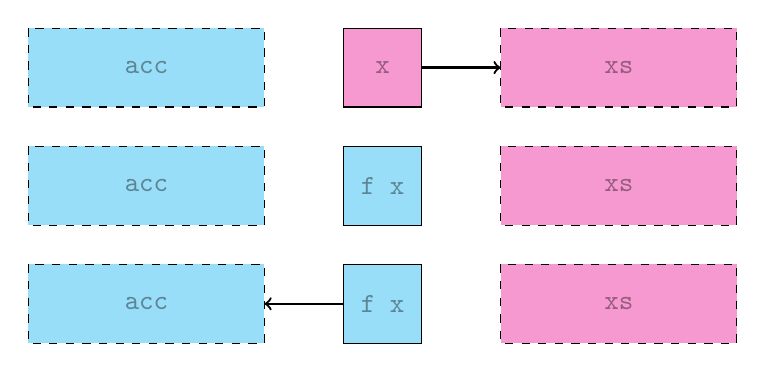
\begin{tikzpicture}[yscale=-1]
    \draw [fill=cyan, fill opacity=0.4, dashed] (0,0) rectangle (3,1) node [pos=.5] {\texttt{acc}} ;
    \draw [fill=magenta, fill opacity=0.4] (4,0) rectangle (5,1) node [pos=.5] {\texttt{x}} ;
    \draw [fill=magenta, fill opacity=0.4, dashed] (6,0) rectangle (9,1) node [pos=.5] {\texttt{xs}} ;
    \draw [thick, ->] (5,0.5) -- (6,0.5) ;
    
    \draw [fill=cyan, fill opacity=0.4, dashed] (0,1.5) rectangle (3,2.5) node [pos=.5] {\texttt{acc}} ;
    \draw [fill=cyan, fill opacity=0.4] (4,1.5) rectangle (5,2.5) node [pos=.5] {\texttt{f x}} ;
    \draw [fill=magenta, fill opacity=0.4, dashed] (6,1.5) rectangle (9,2.5) node [pos=.5] {\texttt{xs}} ;
    
    \draw [fill=cyan, fill opacity=0.4, dashed] (0,3) rectangle (3,4) node [pos=.5] {\texttt{acc}} ;
    \draw [fill=cyan, fill opacity=0.4] (4,3) rectangle (5,4) node [pos=.5] {\texttt{f x}} ;
    \draw [fill=magenta, fill opacity=0.4, dashed] (6,3) rectangle (9,4) node [pos=.5] {\texttt{xs}} ;
    \draw [thick, ->] (4,3.5) -- (3,3.5) ;
\end{tikzpicture}
\end{frame}

\begin{frame}{The \texttt{map} problem: DPS implementation}
\centering
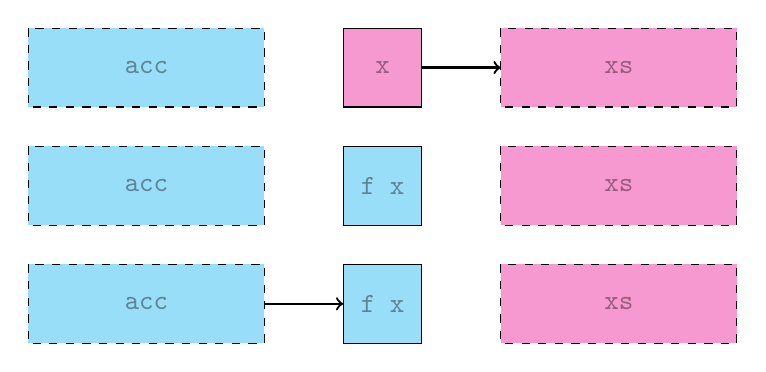
\begin{tikzpicture}[yscale=-1]
    \draw [fill=cyan, fill opacity=0.4, dashed] (0,0) rectangle (3,1) node [pos=.5] {\texttt{acc}} ;
    \draw [fill=magenta, fill opacity=0.4] (4,0) rectangle (5,1) node [pos=.5] {\texttt{x}} ;
    \draw [fill=magenta, fill opacity=0.4, dashed] (6,0) rectangle (9,1) node [pos=.5] {\texttt{xs}} ;
    \draw [thick, ->] (5,0.5) -- (6,0.5) ;
    
    \draw [fill=cyan, fill opacity=0.4, dashed] (0,1.5) rectangle (3,2.5) node [pos=.5] {\texttt{acc}} ;
    \draw [fill=cyan, fill opacity=0.4] (4,1.5) rectangle (5,2.5) node [pos=.5] {\texttt{f x}} ;
    \draw [fill=magenta, fill opacity=0.4, dashed] (6,1.5) rectangle (9,2.5) node [pos=.5] {\texttt{xs}} ;
    
    \draw [fill=cyan, fill opacity=0.4, dashed] (0,3) rectangle (3,4) node [pos=.5] {\texttt{acc}} ;
    \draw [fill=cyan, fill opacity=0.4] (4,3) rectangle (5,4) node [pos=.5] {\texttt{f x}} ;
    \draw [fill=magenta, fill opacity=0.4, dashed] (6,3) rectangle (9,4) node [pos=.5] {\texttt{xs}} ;
    \draw [thick, ->] (3,3.5) -- (4,3.5) ;
\end{tikzpicture}
\end{frame}

\begin{frame}[fragile]{The \texttt{map} problem: DPS implementation}
\begin{adjustwidth}{-1.5em}{-1.5em}
\begin{minipage}{0.5\linewidth}
\begin{lstlisting}
let rec %\textcolor{red}{map\_dps}% %\textcolor{cyan}{dst}% f xs =
  match xs with
  | [] ->
      %\textcolor{olive}{set\_field dst 1 []}%
  | x :: xs ->
      let y = f x in
      let dst' = y :: [] in
      %\textcolor{olive}{set\_field dst 1 dst'}% ;
      %\textcolor{red}{map\_dps}% %\textcolor{cyan}{dst'}% f xs
\end{lstlisting}
\end{minipage}
\begin{minipage}{0.45\linewidth}
\begin{lstlisting}
let map f xs =
  match xs with
  | [] ->
      []
  | x :: xs ->
      let y = f x in
      let dst = y :: [] in
      map_dps dst f xs ;
      dst
\end{lstlisting}
\end{minipage}
\vfill
\begin{lstlisting}
# List.init 250_000 (fun _ -> ())
  |> map Fun.id
  |> ignore
  ;;
- : unit = ()
\end{lstlisting}
\end{adjustwidth}
\end{frame}

\begin{frame}[fragile]{The \texttt{map} problem: TMC}
\begin{lstlisting}
let%\textcolor{olive}{[@tail\_mod\_cons]}% rec %\textcolor{red}{map}% f xs =
  match xs with
  | [] ->
      []
  | x :: xs ->
      let y = f x in
      %\textcolor{cyan}{y ::}% %\textcolor{red}{map}% f xs
\end{lstlisting}
\vfill
\begin{lstlisting}
# List.init 250_000 (fun _ -> ())
  |> map Fun.id
  |> ignore
  ;;
- : unit = ()
\end{lstlisting}
\end{frame}